% !TeX root = ../../thesis.tex
\chapter{背景知識}

\section{深層類神經網路(deep neural network)}

\subsection{簡介}  %
  
深層類神經網路(Deep Neural Network,DNN 或簡稱 NN)又稱「人工類神經網路(Artificial Neural Network,ANN)是來自於神經科學家麥氏(McCulloch)與皮氏(Mitts)等人在 1943 年提出 \cite{mcculloch1943logical},取法自生物神經連結的計算模型。以發展此類模型為主軸的心理學流派,在計算認知神經科學中被稱為「連結派(Connectionism)」,旨在模擬生物神經系統的連結,以模仿生物的各項功能。爾後在工程界進而透過機器學習的最佳化演算法,使得整個模型能夠藉由資料去貼合(Fit)理想的函數,以達成應用或工程上所需要的各種任務。因為該類網路的彈性與計算上易於平行化的特徵,能夠很恰當的利用諸如圖形處理器(Graphics Processing Unit,GPU)等硬體裝置的優勢,以求更好的描述資料分佈、達到前所未有的效能,因此近年在電腦科學的機器學習領域中獲得重大進展,現已成為人工智慧發展的主流。

深層類神經網路最基本的單位是「神經元(Neuron)」,模仿生物神經細胞接收訊號、處理到傳出的過程,每個神經元會接收一串數字作為輸入並計算出一個數字作為輸出,可用下列向量運算的式子描述:
$$y=\sigma(w^\top x + b) $$
其中 $x$ 是 $N$ 個輸入的數字,可描述為一個 $N$ 維的向量;$w$ 為該神經元對每個輸入值給予的權重,再對加權平均後的結果加上偏差值 $b$ 後,經過激發函數(Activation Function)$\sigma$ 的非線性轉換後最後得到輸出。其中常見的激發函數有線性整流單元(Rectified Linear Unit,ReLU)、S 函數(Sigmoid Function)或雙曲正切函數(Hyperbolic Tangent Function,$\tanh$)等等。

\begin{figure}
    \centering
    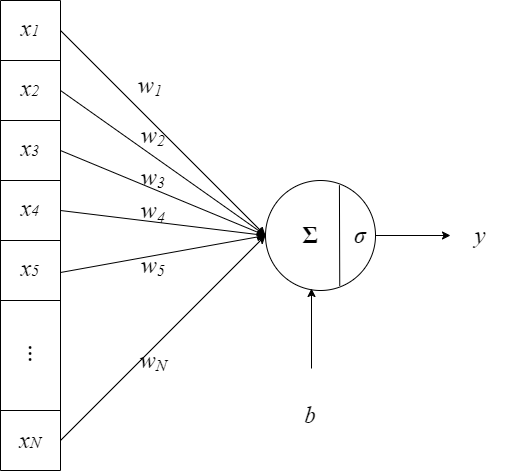
\includegraphics[width=0.5\linewidth]{figures/neuron.drawio.png}
    \caption{神經元示意圖}
    \label{fig:single-neuron}
\end{figure}

由多個神經元可形成單層感知機(Perceptron) \cite{rosenblatt1958perceptron},為了能夠處理更複雜的運算,多層感知機(Multi-layer Perceptron,MLP)被提出。透過梯度下降等演算法進行最佳化,以降低網路輸出與目標函數之間的誤差,再將此誤差藉由反向傳播演算法對整個網路的權重進行調整,以最好的擬合想要的函數。

基於深層類神經網路延伸,常見的網路架構包含卷積式(convolutional)、遞迴式(recurrent)與轉換器(Transformer)類神經網路等類別。由於這些架構在語音與文字處理上的廣泛應用,因此在下面分別介紹:

\subsection{卷積式(convolutional)類神經網路}  

卷積式類神經網路(convolutional neural network)為 1998 年由楊氏(LeCun)提出 \cite{726791},旨在利用訊號處理上卷積(convolution)的運算模擬人類視覺皮質感知 \cite{hubel1959receptive} 的特性,利用其移動不變性(shift-invariance)來捕捉二維影像中的局部(local)特徵,以便於後續的類神經網路可以對輸入的資料進行更整體而全面的判斷。

% 這邊是不是要處理不同 features
在語音處理的領域中,有別於影像的二維資料,語音訊號的資訊是被呈現在時間軸的維度上,因此通常使用一維的卷積式類神經網路,以模仿人耳聽覺對時變訊號的窗框(window)處理過程,讓模型可以觀察到輸入語音在不同解析度(resolution)上的資訊,例如本研究特別著重的音位(phoneme)等。


\subsection{遞迴式(recurrent)類神經網路}  

遞迴式類神經網路主要用於處理序列資訊,因此在語音處理和自然語言處以中

\begin{figure}
    \centering
    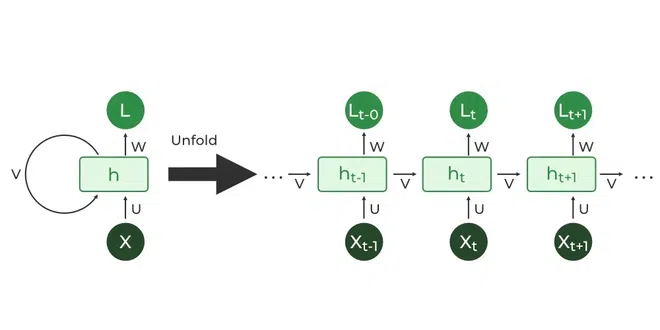
\includegraphics[width=0.5\linewidth]{figures/image.png}
    \caption{RNN}
    \label{fig:RNN}
\end{figure}

\subsection{序列至序列(sequence-to-sequence)模型}  


% long-term dependency
由於許多語言相關的資料都是兩個序列之間互相配對的關係,包含語音和文字等時序訊號等等,都是以時間軸為主要資料呈現的維度。因此這類資料通常會使用序列至序列的模式進行訓練,旨在模擬輸入與輸出序列之間的變化與相依關係(dependency)。

此類模型一般的架構是由一個編碼器(encoder)和一個解碼器(decoder)構成,其中編碼器是將輸入訊號藉由內部表徵(latent representation)進行編碼,依據每個時間點輸入訊號的變化來調整其內部表徵狀態,接著將最後一個時間點的表徵作為整個序列的代表,傳遞給解碼器生成輸出訊號的序列。

\subsection{專注(attention)機制}  

為了解決序列至序列模型中的長期依賴問題,專注機制被提出


原本的序列自序列模型本身。 需要讓解碼器單純透過最後一個時間 點。 的表征資訊來完全儲存輸入序列的一切資訊 以工解碼器判斷。 并生成輸出序列。 然而,由于 單就最後一個向量進行判斷對於解碼器而言過於不易。因此。 盧氏提出。 在編碼器中對輸入序列的不同時間點進行注意力機制 亦即讓解碼器可以根據當下 所需要輸出的 內容判斷應該要重新對輸入序列的哪些部份 進行更多的加權 。

\subsection{轉換器(Transformer)}

其後,由瓦氏(Vaswani) cite 提出的 論文中 提出了一個完全由注意機制。 所構成的序列自序列模型。 原先該模型適用於解決機器翻譯。 的問題。
由於其能夠高度平行化的特性, 日後在 自然源處理和語音處理,甚至到電腦視覺領域等近乎整個深層學習的領域都被廣泛的應用。



\section{表徵(representation)學習與自監督式學習(SSL)}

\subsection{特徵}

原本在文字和語音。文字會用 TF-IDF 等等,語音則會用 mel 和 MFCC

\subsection{表徵學習}

後來基於 Mikolov 的 Word2Vec
word2vec 是 mikolov \CITEME 最早提出跟對於文字進行語義表徵的 work。在其後
開始嘗試從大量資料去學習出表徵

結合 contextulaized embedding 有了 ELMo

\subsection{自監督學習(self-supervised learning,SSL) (這邊接下來直接看以前碩論怎麼分。宏毅的再說)}

從 contextulaized 的精神,結合 SAttn,BERT 被提出來,並有了 SSL 的概念

SSL 的好處是可以更好的利用 NN 的學習與泛化(generalization)能力,從大量的未標註資料中,就由 pretext tasks 的引導,在 unsupervised 的情形下利用資料本身結構進行學習。

(提到「提出了很多語音基石模型」)

\subsubsection{重建式學習}

BERT
以重建被
遮罩語言模型

\subsubsection{預測式學習}

GPT
APC


\subsubsection{對比式學習}

CPC // 所以這個在後面會不會出事?

\subsection{向量量化(vector quantization)}



\subsection{無文字(textless)與離散單元}




\section{本章總結}


